\documentclass[a4paper,man,natbib]{apa6}
\usepackage{microtype}
\usepackage{mathtools} % needed
\usepackage{hyperref}
\usepackage{tabularx}
\newcolumntype{Y}{>{\raggedright\arraybackslash}X}
\usepackage[normalem]{ulem}
\hypersetup{hidelinks=True}
\newcommand*{\smex}[1]{\textit{#1}} % 'small example'
\newcommand*{\spex}[1]{``{#1}''} % 'spoken example'
\newcommand*{\term}[1]{\emph{#1}} % introducing a new term
\newcommand*{\citegen}[1]{\citeauthor{#1}'s~(\citeyear{#1})}
\newcommand*{\SE}{\mathit{SE}} % fix funny "SE" spacing
\newcommand{\resultsLog}[3]{$\beta = #1$, $\textnormal{SE} = #2$, $p #3$}
\newcommand{\resultsLM}[3]{$\beta = #1$, $\textnormal{SE} = #2$, $t #3$}

\title{Such gesture, very lie, wow}
\author{reorder(MC,JK,JL)}
\affiliation{Psychology, PPLS, University of Edinburgh}
\ifapamodeman{\note{\begin{flushleft}%
Josiah King\\
Philosophy, Psychology and Language Sciences\\
University of Edinburgh\\
7~George Square\\
Edinburgh EH8~9JZ, UK\\[1ex]
\url{J.P.J.King@sms.ed.ac.uk}
\end{flushleft}}}

\abstract{
Previous research suggests that, when questioning the veracity of an utterance, we perceive certain non-linguistic behaviours to indicate that a speaker is being deceptive.
Recently, work has highlighted how listeners' associations between speech disfluency and dishonesty happen at the earliest stages of reference comprehension, suggesting that contextual information about the manner of spoken delivery influences pragmatic judgments simultaneously with integration of lexical information.
The studies presented here ask whether listeners also rapidly integrate the visual channel in making judgments about a speaker's honesty.
Eye- and mouse-tracking experiments investigate the time-course of pragmatic judgments on whether or not a speaker is being deceitful, when faced with different visual cues to deception.
Participants saw and heard a video of a potentially dishonest speaker describe treasure being hidden behind a named object, while also viewing both the named object and a distractor object. 
Their task was to click on the object behind which they believed the treasure to actually be hidden.
Experiment 1 investigates the speed with which listeners associate visual cues with deception, using a variety of static and dynamic cues.
Experiment 2 establishes a dishonesty-bias for adaptor (fidgetting) gestures, and asks whether listeners' judgments of deception correlate with how nervous they think the speaker appears in each video.
Results show that the visual modality can have a rapid and direct influence on pragmatic judgments, supporting the idea that communication is fundamentally multimodal, and should be studied as such.
The emergence of deception-judgments based on visual cues appear to be more gradual than in previous studies resarching spoken cues.
}


\begin{document}

\shorttitle{What do liars look like?}
\maketitle
\linenumbers
\noindent
That people deceive one another is an inescapable aspect of everyday communication.
After studying participants' social interactions over a one week period, \citet{DePaulo1996} concluded that people lie on average twice a day.
The idea that it possible to detect deceit --- that there are systematic differences in people's behaviour depending on whether they are telling a truth or a lie --- has long captivated human interest in a variety of areas, from criminal interrogations to the business world.\footnote{Where, in some cases, ``how to lie'' is equally as important. See https://www.marketplace.org/2008/02/18/busness/lying-essential-doing-business}
Much research has investigated the behaviours that listeners associate with lying, covering a wide range of multi-modal phenomena from speech disfluencies and vocal pitch to visual cues such as postures and hand movements.
Few studies, however, have studied the time-course of inferences to deception, and fewer still have done so in a multi-modal setting.
The present experiments investigate listeners' associations of a speaker's non-verbal behaviour with the veracity of an utterance, studying how and when visual information about a speaker is integrated in to the pragmatic interpretation of speech.


In most natural communication, speakers can convey information via multiple channels.
Along with spoken delivery, a speaker's gestures, postures and facial expressions, are all available information which may be used to influence pragmatic judgements such as that of the (dis)honesty of an utterance.
In an analysis of 33 studies, \citet{Zuckerman1981} found that nine out of the ten visual cues-to-deception that were included in the analysis were believed to be indicative of deceit. 
In a further subset of 13 studies reporting relationships between cues and subsequent deception judgments (rather than explicit beliefs about cues), three of the four available visual cues were associated with judgments of deception.
The visual cues which listeners associated with deception appear to follow a trend, with more movement signalling dishonesty.

Interestingly, listeners appear to hold these associations and beliefs despite the reliability of cues as actual signals of deception being inconclusive: \citet{Zuckerman1981} did find that more shrugs and fidgetting be indicative of deceit, but a more recent meta-analysis \citet{DePaulo2003} found little evidence of a relationship between lying and most forms of movement.
Furthermore, some studies have found deception to be associated with a \emph{decrease} in hand, arm, and leg movements \citep[e.g.][]{DePaulo1992, Ekman1989, Vrij1995}, as well as a reduction in illustrative gesturing \citep[e.g.][]{DePaulo2003, Cohen2010}.
Even speakers' post-hoc perceptions of their own gestures when lying have been found to be at odds with how they actually behaved:
Speakers believe themselves to move more \citep{Vrij1996} as well as to be more disfluent \citep{Zuckerman1981a}.
\citet{Vrij1996} found that after partaking in two interviews --- one in which they were truthful, the other dishonest --- participants believed that their movements increased when lying, even though a decrease actually occurred (whether or not participants were informed before-hand that deception is usually associated with a decrease in movements had no effect).

All this suggests that the links which listeners' draw from visual information to deception might not be due to learning these associations from experience.
What is more, in everyday communication, there are few occurrences where listeners are given immediate feedback on the honesty of a given utterance.
Why then do listeners' hold such strong associations and beliefs between visual cues and lying?
One suggestion \citep{DePaulo1982} is that this association is based on a set of cues which listeners consistently associated with deception via a rule-of-thumb based heuristic.
This set of cues may be predicated on lay beliefs about deception, or on introspection as a speaker rather than experience as a listener, but ultimately leads to the somewhat innaccurate model of what deceitful behaviour looks and sounds like. 

%Evidence for a rule-of-thumb association between certain cues and deception can be found 
%the link between movement and deception follows a simple, straightforward rule-of-thumb based approach.

Recent research by \citet{Loy2017} investigating the time-course of the association between lying and speech disfluency supports the idea that this rule-of-thumb based approach is present when manner of spoken-delivery influences judgments of deception.
\citet{Loy2017} used a visual world paradigm in which participants were presented with two objects along with utterances describing the location of some treasure purportedly hidden behind one of the objects.
These utterances were presented as having been elicited in a previous experiment, and could be either truthful or dishonest.
Crucially, \citet{Loy2017} manipulated the manner of spoken delivery, with half of the experimental items containing a speech disfluency.
Participants were tasked with choosing where they \textit{believed} the treasure to really be hidden --- the object named in the utterance (indicating a judgment of honesty), or a distractor (indicating dishonesty).
Participants were more likely to judge disfluent utterances as dishonest than fluent ones (as indicated by more clicks on the distractor on disfluent trials). 
Importantly, their results showed an early bias in both eye and mouse movements towards the non-referent object, suggesting that speech disfluency is already incorporated into the model of the speaker, having an immediate effect on their interpretation of the utterance. 

Little is known, however, about whether such rapid integration of cues might extend to the visual channel of communication. 
To adhere to a rule-of-thumb based association between, for example increased movement and lying, would result in potentially over-attributing any movements a speaker might make as a signal of deception. 
Co-speech movements are substantially more varied than speech disfluencies, and can be attributed to many things, some only indirectly related to the production of speech (e.g. ?).%JK 
An alternative account of how non-linguistic information might influence listeners' judgments of deception involves a form of speaker-modelling.
It might be that, when presented with a possibly deceitful utterance, listeners infer information about a speaker's metacognitive state, suggesting that visual and spoken cues are linked to deception via the perception of, e.g. nervousness, or cognitive effort. 
%link car-horns in here?
Such an account is more computationally demanding, and the link from a given movement to a judgment of deception would likely take more time to establish, as it requires reasoning about the cause/intention of the movement.%JK reword

To date, the link between visual cues and perceived deceit has been studied only in terms of after-the-fact judgments, or assessing listeners' explicit beliefs about cue validity (see \citealt{Vrij1996a, Zuckerman1981a}).
Studying the time-course of judgments of a speaker's honesty when presented alongside different visual cues can help to shed light on how these cues are integrated into pragmatic judgments such as that of deception.
We extend the `treasure game' paradigm from \citet{Loy2017} to include a video of the potentially deceptive speaker describing the location (behind one of two objects) of some hidden treasure on the screen while listeners attempt to guess the true location based on whether they believe the speaker to be lying or telling the truth. 
%%% Jia: we should include a figure of the display here %%%
Crucially, we manipulate the presence or absence of visual cues in the video.
Experiment 1 investigates how the time-course of deception-judgments varies between different types of cues, including both increases in movement and different static postures.
If listeners associate visual cues with deception via a rule-of-thumb association between movement and deception, then a bias towards the not-referred to object should occur early on following trials in which the speaker moves.
In Experiment 2 we focus on the association between lying and adaptor gestures (fidgeting movements), asking whether listeners' judgments are predicted by their perceptions of how nervous they think the speaker to be in each video.

\section{Experiment 1}
Experiment 1 makes use of eye- and mouse-tracking to investigate the time course of listeners' judgments about the honesty of an utterance, and how these judgments are influenced by the occurrence of various visual cues. 
The experiment was presented as a `lie detection game', with each trial presenting a video of a potentially deceptive speaker describing the location of some hidden treasure on the screen (behind one of two possible objects). 
Participants are tasked with clicking on where they believe the treasure to be hidden based on their judgement of the speaker's honesty.
We employ 3 types of visual cues --- trunk movements, adaptor gestures, and different postures --- and investigate whether listeners associate any of these with deception.
%% (add) Our results show that...

%JK 
%The three types of visual cue provided distinct sets of stimuli when paired with speech. 
%Trunk movements were completed in entirety prior to speech onset, providing an utterance-initial visual cue.
%Adaptor gestures were completed during the presentation of speech, creating an utterance-medial cue.
%The different postures provided a more `global' cue ?? %JK reword..


\subsection{Materials}
Visual stimuli consisted of the same 120 line drawings from \citet{Snodgrass1980} which were used in \citet{Loy2017}, presented in pairs across sixty trials. 
In each trial, the speaker named one object (referent) as that which concealed the treasure; the other object is hereafter named the distractor.
Each referent was associated with a recording specifying the image as the object that the treasure was hidden behind (``The treasure is behind the <referent>'').
Along with these images, each trial contained a video of a person who was purported to be the speaker of the utterances. 
So that videos could be counterbalanced across referents, and thus across utterances, the face of the person in the video was blurred. 
This meant that, when presented with a given utterance, it was believable that both audio and visual stimuli had been produced concurrently. 

Sixty videos (30 Cue, 30 No-Cue) were created. 
The thirty no-cue videos were comprised of ten recordings (each presented thrice) of a speaker sitting motionless with her hands either side of a tablet on a table, upon which the location of treasure was purported to be displayed.
Ten videos presented the speaker making one of five trunk movements, ten presented various adaptor gestures (e.g. finger tapping, head tilts), and ten presented the speaker sitting motionless but in a different posture to that of the no-cue videos (e.g. hand on chin, arms crossed, etc).

In order to make the stimuli look as natural as possible, a variable video-to-speech-onset was adopted for the 30 cue videos.
For trunk movements, the frame at which the movement ended was identified and used as the point of utterance onset (Mean onset = 1430ms, SD = 440ms).
This allowed the duration of the trunk movement to be interpretable as speech initiation time, which could in turn potentially be associated with the speaker preparing a dishonest utterance.
To control for any sensitivity to the duration of pre-utterance video, these durations were matched in the no-cue videos.
For adaptor gestures, the movements overlapped with speech, with the duration of overlap determined individually for each video (Mean = 1370ms, SD = 410ms).
These durations were matched in the videos that presented the speaker sitting in a different posture.

As with \citep{Loy2017}, 20 critical referents were counterbalanced across two lists, each containing 10 cue and 10 no-cue videos.
The 10 cue videos were trunk movements since we predicted these to be the most likely visual cue to elicit judgements of deception\citep{Vrij1996a}
%Jia: think we should try and provide a cite for this (one of the Vrij studies?)
% JK: have done, but it's not great. Vrij splits "trunk movements" (moderate assocation) and "postural shifts" (strong association). I think we used trunk movements to mean postural movements. It's not clear what Vrij uses. 
The remaining 40 referents were randomly paired with one of the remaining videos (10 adaptors, 10 different postures, 20 no-cue) for each participant, with no repetition of referents across videos.

\subsection{Procedure}
Stimuli were displayed on a 21~in.\@ CRT monitor, placed 850~mm from an Eyelink~1000 Tower-mounted eye-tracker which tracked eye movements at 500~Hz (right eye only). 
Audio was presented in stereo from speakers on either side of the monitor. 
Mouse coordinates were sampled at the frame rate of the videos (25~fps). 
The experiment was presented using OpenSesame version~3.1 \citep{Mathot2012}.
Eye movements, mouse coordinates and object clicked (referent or distractor) were recorded for each trial.

Figure \ref{fig:v1_trial} presents a sample trial from the experiment. 
\begin{figure}[Ht]
  \centering
	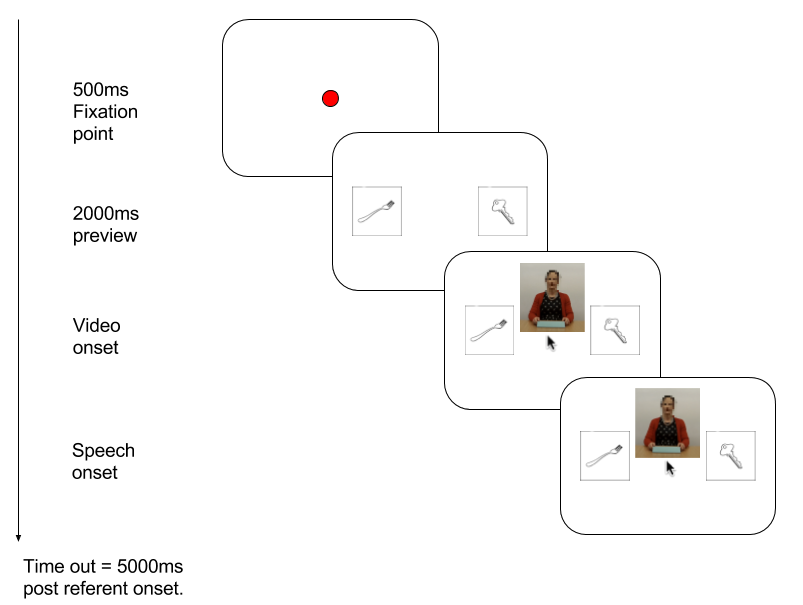
\includegraphics[width=\linewidth]{./img/e7_trial.png}
  \caption{Procedure of a given trial, Experiment 1}
  \label{fig:v1_trial}
\end{figure}
Between trials, participants underwent a manual drift correct, after which the fixation dot turned red for 500ms. 
After this, the two objects (referent and distractor) were displayed on the screen for 2000ms.
The video then appeared and the cursor was centred and made visible.
Playback of the utterance began after the variable speech onset associated with each video (Mean = 1410ms, SD = 410 ms). 

The instructions emphasised that the videos participants saw were recorded from a previous experiment, in which the speaker had to describe the location of some hidden treasure with the aim of misleading the listener into choosing the wrong location.
Participants were instructed to click on the object behind which \textit{they believed} the treasure to be hidden, with the overall aim of accumulating as much treasure as they could across the experiment.
Participants received no feedback after their object clicks, except on bonus trials, which are described in the next section.

Participants completed five practice trials (one of which was presented as a bonus round) prior to the main experiment. 
Two of these were static, two displayed the speaker in different postures, and one displayed the speaker making a trunk movement.

\subsection{Bonus Rounds}
To maintain motivation throughout the study, participants were told that there were a number of ``hidden bonus rounds'' which offered more treasure than regular rounds.
25\% of trials (half in the cue condition; half in the no-cue condition) were randomly designated as bonus rounds for each participant.
These trials were visually identical to regular trials, with the exception of a message informing participants that they had successfully located bonus treasure following their mouse click (regardless of the object chosen).

Participants were also told that the top scorers would be able to enter their names on a high-score table, which was shown at the beginning of the experiment. 

\subsection{Post-test Questionnaire}
Participants were asked to complete a short post-test questionnaire. 
The questionnaires contained three questions, the most important of which asked if participants noticed anything odd about the visual or audio stimuli.
Any participant who indicated that they noticed anything unusual was then verbally questioned, to decide whether they believed that the speech and gesture had been produced naturally and simultaneously.
All participants were subsequently debriefed (told that the audio and video were created separately and stitched together), and asked again verbally if they noticed anything unusual in that respect. 

\section{Results}
Twenty-four native English speaking participants took part in the experiment for a desired sample size of twenty. 
Participants were recruited from the University of Edinburgh community, and participated in return for a payment of \pounds{}4.
Data from four participants who indicated suspicion of the proposed origins of the audiovisual stimuli based on the post-test questionnaire were removed from all analyses.

\subsection{Analysis}
Analysis was carried out in R version~3.4.4 \citep{Rbase2017}, using the lme4 package \citep{Bates2015}. 
Trials in which participants did not click on either the referent or distractor (0.003\% of trials) were excluded from all analyses. 

Object clicked (referent or distractor) was modeled using mixed effects logistic regression, with fixed effects of cue type (No-Cue, Different Postures, Trunk Movements, Adaptor Gestures) and video-to-speech duration (Z-scored), thus controlling for any possible effect of perceived speech latency on judgments of dishonesty.
Random intercepts and slopes for cue type and video-to-speech were included by-participant, along with random intercepts by-referent.
Reaction times (measured from referent onset) were modelled with the same fixed and random effect structure.
Following \citet{Lo2015}, we compared mixed effects logistic regression models which specified an identity link function, assuming gaussian, gamma and inverse gaussian distributions.

In previous studies using the treasure game paradigm, eye- and mouse- movements have been analysed over the time window starting at the onset of the referent name and extending for 800~ms; just beyond the duration of the longest referent (776~ms). 
Because the current study includes in the analysis all available referents (rather than the subset used in previous experiments), this window is extended to 0--1100~ms to include the duration of the longest referent (1062~ms).

Eye fixation data was averaged into 20~ms bins (of 10 samples) prior to analysis.
For each bin, we calculated the proportions of time spent fixating referent or the distractor, resulting in a measure of the proportions of fixations on either object over time.

The position of the mouse was sampled every 40~ms.
Using the $X$ coordinates only, we calculated the number of screen pixels moved and the direction of movement (towards either referent or distractor).
We then calculated the cumulative distance travelled towards each object over time as a proportion of the cumulative distance travelled in both directions up until that time bin.
Movements beyond the outer edge of either object were considered to be `overshooting' and were not included in calculations (0.8\% of samples).
Eye- and mouse- biases were calculated from the proportions of referent to distractor fixations, and were subsequently empirical logit transformed \citep{Barr2008}. 
In these measures, a value of zero indicates no bias towards either object, and positive and negative values indicate a bias towards the referent and distractor respectively.

Eye and mouse data was modelled over the time window from 0 to 1100~ms post-referent onset using linear mixed effects models, with fixed effects of time, cue type, and their interaction.
Random intercepts and slopes for time were included both by-referent and by-participant, along with by-participant random effects of cue type.
Following \citet{Baayen2008}, we considered effects in these models to be significant where $|t|>2$.

%JK Maybe just get rid of this >>
As visual inspection of the time-course of fixations towards either object suggested that there was a later effect of visual cues in participants' decision of which object to click on, growth curve analysis (See \citealt{Mirman2008}) was used to investigate this further. 
This analysis was conducted over the time window from 0 to 1815~ms post-referent onset included 3 degrees of orthogonal polynomials for time, based on the pattern of the elogit referent-distractor bias having 2 turning points. 
These time polynomials, along with their interaction with cue type, were included as fixed effects in a linear mixed effects model, with random intercepts and slopes for all time polynomials both by-participant and by-referent.


\subsection{Object clicks} 
Across the experiment, participants clicked on the referent in 55\% of trials and the distractor in only 45\%.
Table \ref{table:v1_clicks} shows the percentage of clicks across all participants to either object following different types of visual cue.
When presented with an utterance accompanied by no-cue, participants showed a bias toward a final interpretation of the utterance as truthful, with more clicks to the referent than the distractor \resultsLog{0.62}{0.16}{<0.001}.
Analysis by individual cue type showed that all visual cues resulted in a reduction of this bias, with adaptor gestures (\resultsLog{-1.03}{0.34}{<0.005}) showing a greater change than different postures and trunk movements (\resultsLog{-0.72}{0.31}{<0.05} and \resultsLog{-0.62}{0.26}{<0.05} respectively). % Jia: just to make it clear that it was a separate model for each gesture type, otherwise talking about it in terms of 'greater change' sounds like it was just one model
%JK not sure what you mean? it was one model, with gesture type as a predictor (e.g. coefficients for each level of gesture type represent difference from baseline (no-gesture)). admittedly, can't say that effect of adaptors is signif > effect of postures.
The duration of video shown prior to the beginning of speech was not found to be associated with which object was eventually clicked.

Comparisons --- via both AIC and BIC --- of reaction time models suggested that an inverse gaussian distribution provided the best fit to the observed data.
Neither cue type nor duration of video prior to speech was associated with a significant change in reaction times.

\begin{table}
\caption{Breakdown of mouse clicks recorded on each object (referent or distractor) by type of visual cue for Experiment 1}
\label{table:v1_clicks}
\begin{tabularx}{\linewidth}{YYYYY}
\hline
& No-Cue & Different Posture & Trunk Movement & Adaptor Gesture \\
Clicks to Referent & 63.8\% & 48.0\% & 49.7\% & 41.5\%  \\ 
Clicks to Distractor & 36.2\% & 52.0\% & 50.3\% & 58.5\% \\
\hline
\end{tabularx}
\end{table}

\subsection{Eye movements}
Figure \ref{fig:v1_eye} shows the time-course of fixations to referents and distractors over 2000~ms from referent onset, split by each type of video.

Analyses conducted over the period from referent onset to 1100~ms post-onset (duration of the longest referent) showed that, when presented with a no-cue video, participants displayed a fixation bias towards the referent which increased over time (\resultsLM{1.15}{0.29}{>2}).
For videos which presented the speaker either in a different posture, or producing an adaptor gesture, this increasing bias to the referent was significantly reduced
(\resultsLM{-0.97}{0.13}{>2}, \resultsLM{-0.59}{0.13}{>2}), but this was not the case for videos of trunk movements (\resultsLM{-0.25}{0.15}{=1.67}). 

Growth curve analysis over the period from referent onset to 1815~ms post-onset (mean click time) showed that when presented with a no-cue video, participants showed an tendency to fixate on the referent over the course of this time period (\resultsLM{0.67}{0.11}{>2}). %intercept term
Significant effects of cue type on the intercept term indicated lower overall referent fixations during this period after viewing a different posture (\resultsLM{-0.36}{0.04}{>2}), a trunk movement (\resultsLM{-0.29}{0.4}{>2}), or an adaptor gesture (\resultsLM{-0.67}{0.4}{>2}), in comparison to the no-cue videos.
Significant interactions of cue type and the linear time coefficient indicate that this reduction in referent-bias dependent on cue type increases over the course of the window, with adaptor gestures showing a larger reduction relative to no-cue videos (\resultsLM{-116.89}{11.62}{>2}) than different postures (\resultsLM{-75.41}{11.65}{>2}) and trunk movements (\resultsLM{-58.78}{12.97}{>2}). 
% JK: Beyond this, different posture videos showed a more gradual initial tendency towards the referent relative to the no gesture videos (\resultsLM{39.83}{11.64}{>2}) and trunk movement videos showed an increased ?? -- the little curve at the end.. (\resultsLM{33.50}{12.75}{>2}).
Figure \ref{fig:v1_gca} shows the time-course of the elogit referent-distractor bias, alongside the fitted values from the growth curve model. 

\begin{figure}[Ht]
  \centering
	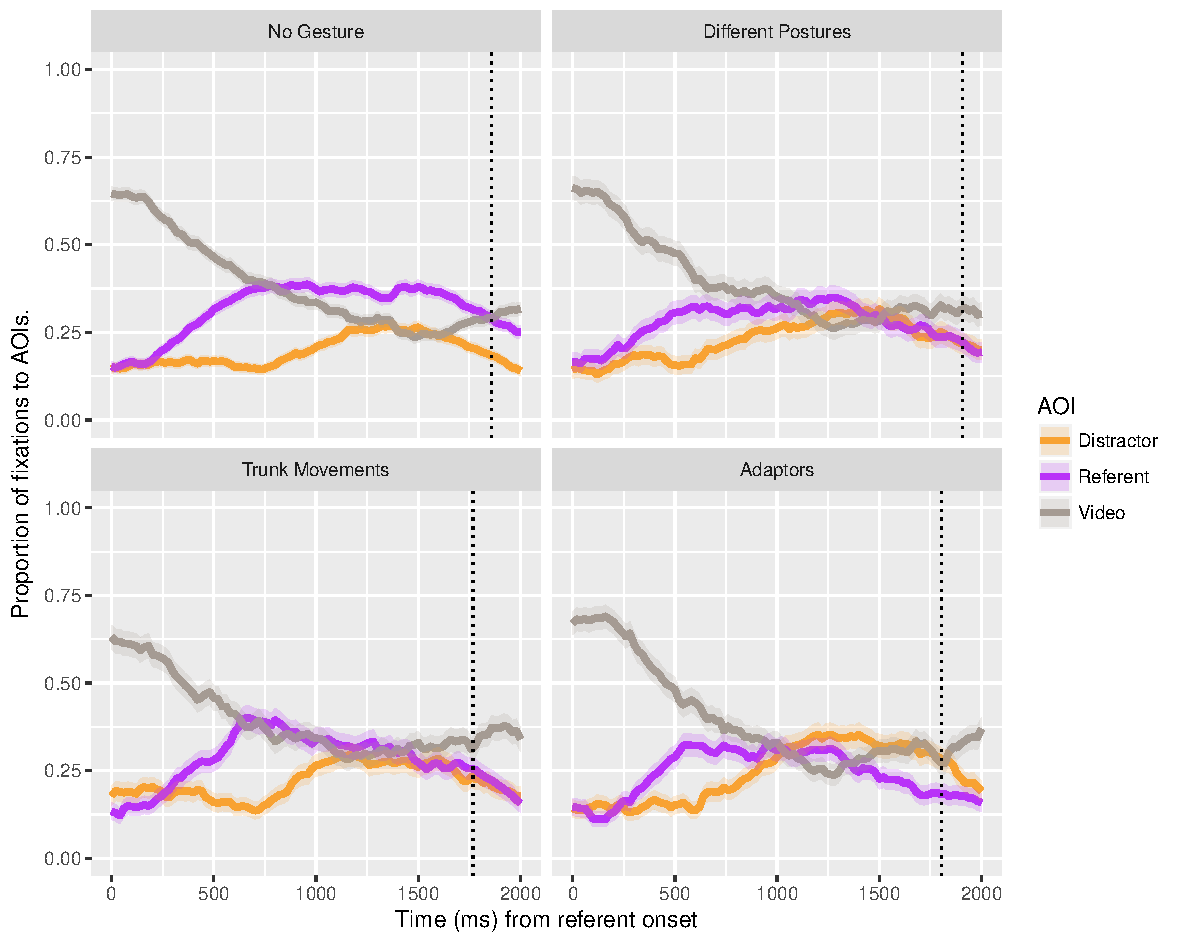
\includegraphics[width=\linewidth]{./img/e7_fixations.pdf}
  \caption{Eye-tracking results for Experiment 1: Proportion of fixations to each object (referent, distractor, video), from 0 to 2000 ms post-referent onset, calculated out of the total sum of fixations for each 20~ms time bin. Shaded areas represent $\pm$ 1 standard error of the mean.}
  \label{fig:v1_eye}
\end{figure}

\begin{figure}[Ht]
  \centering
	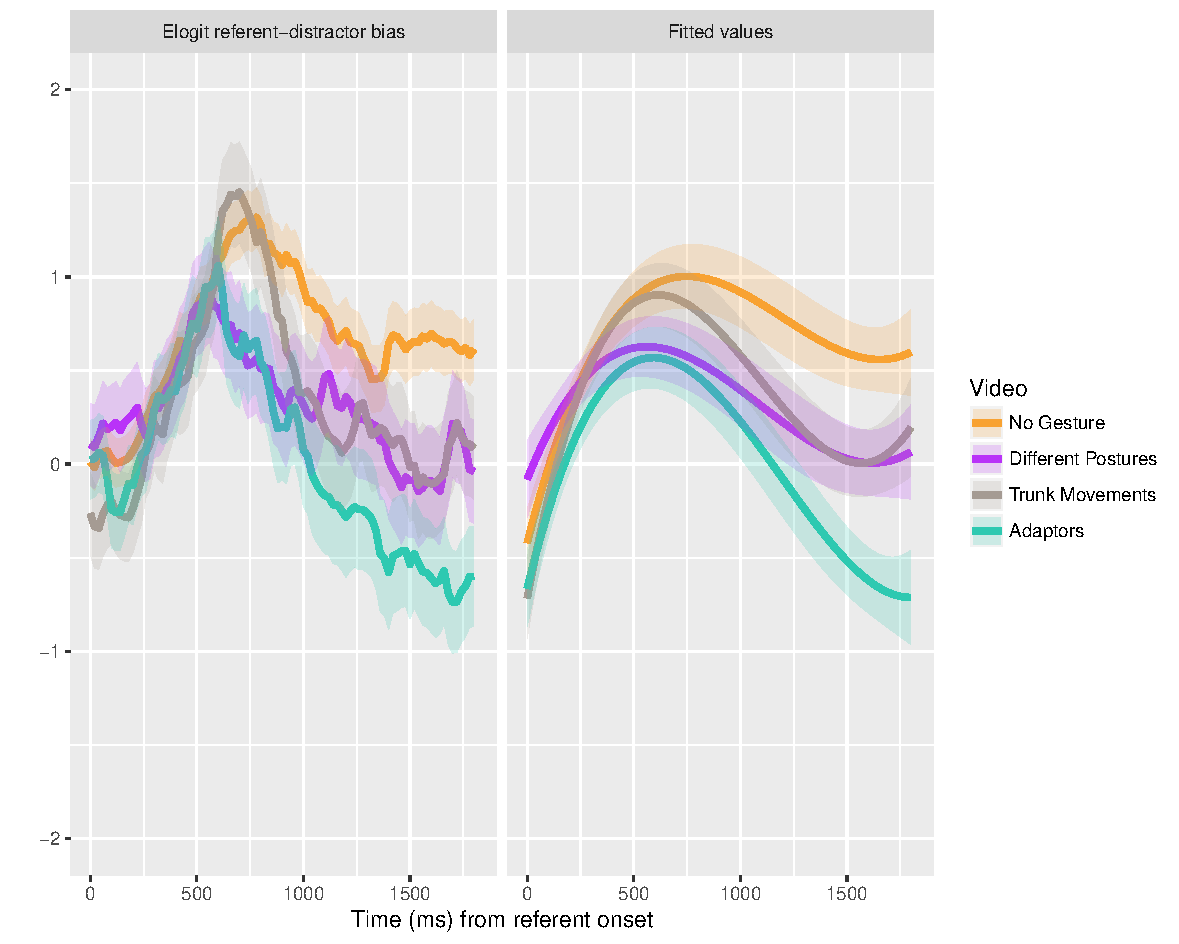
\includegraphics[width=\linewidth]{./img/e7_gcamodel.pdf}
  \caption{Elogit referent-distractor bias, and fitted values from growth curve analysis}
  \label{fig:v1_gca}
\end{figure}


\subsection{Mouse movements}
Figure \ref{fig:v1_mouse} shows the time-course of the proportions of cumulative distance the mouse moved towards the referent and distractor for 2000~ms from referent onset, split by each type of video.
Analysis on the time window from 0 to 1100~ms post-referent onset patterned with the eye-tracking data:
When viewing a speaker making no visual cue, participants showed an increasing tendency to move towards the referent over this period (\resultsLM{1.08}{0.22}{>2}).
As with the eye-movements, different postures and adaptor gestures resulted in a weakening of this referent-bias (\resultsLM{-0.81}{0.13}{>2} and \resultsLM{-0.77}{0.13}{>2} respectively), but trunk movements did not (\resultsLM{-0.10}{0.14}{=0.69}). 

\begin{figure}[Ht]
  \centering
	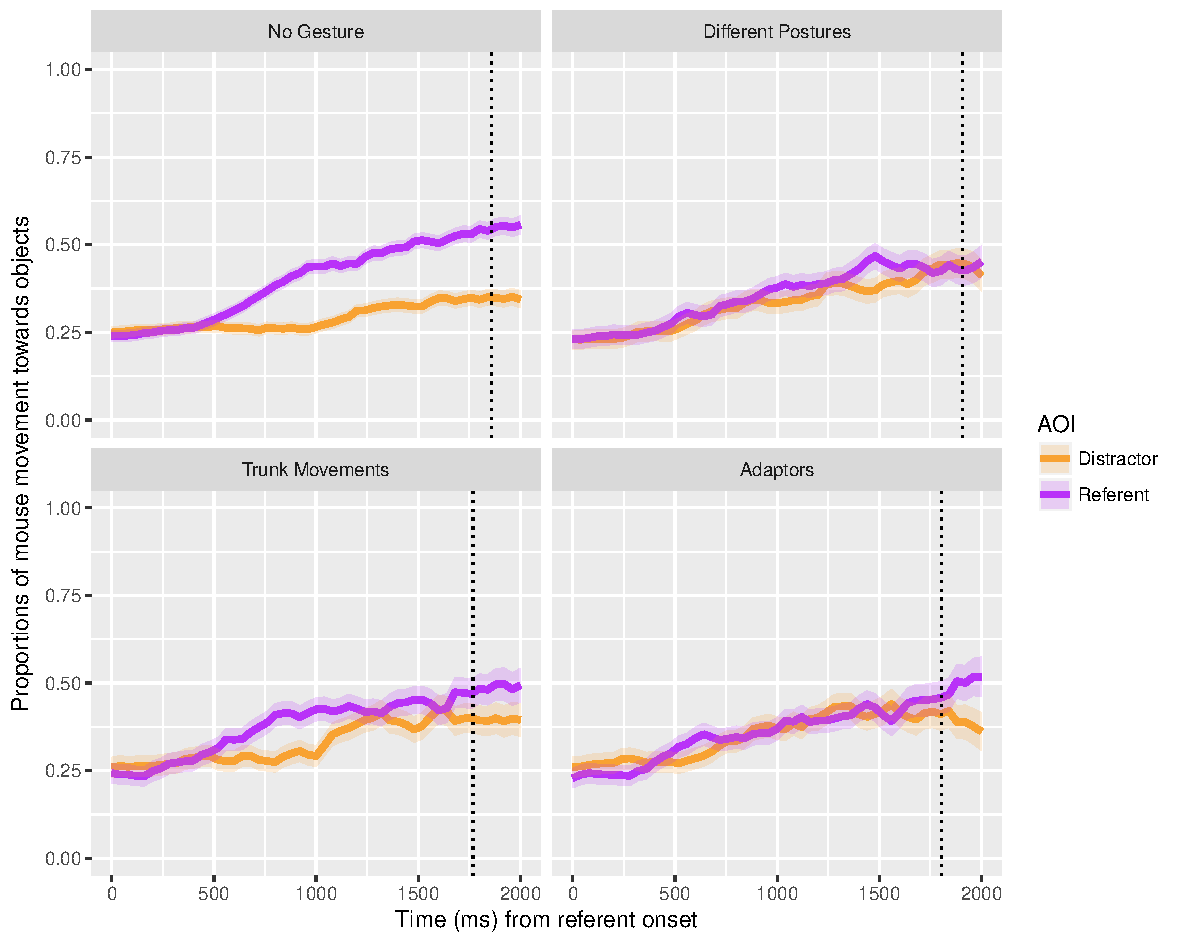
\includegraphics[width=\linewidth]{./img/e7_mouset.pdf}
  \caption{Mouse-tracking results for Experiment 2: Proportion of cumulative distance traveled toward each object from 0 to 2000 ms post-referent onset. Proportions were calculated from the total cumulative distance participants moved the mouse until that time bin (from video onset, when cursor was made visible). Shaded areas represent $\pm$ 1 standard error of the mean.}
  \label{fig:v1_mouse}
\end{figure}


\section{Discussion}
Experiment 1 investigated how the pragmatic inferences listeners make about a speaker's honesty are influenced by the presence of different types of movements and postures. 
As in previous studies using this paradigm (minus the video component) \citep{Loy2017, King2018}, participants showed a tendency to interpret an utterance as truthful when it had been presented without any potential cue to deceit.
Utterances presented alongside any cue --- both movement and different postures --- weakened this tendency, but only the presence of adaptor gesturing resulted in significantly more judgments of deception than truthfulness (indicated by more clicks to the distractor over the referent).

The influence of the visual channel was also evident in participants' early stages of utterance processing. 
Across videos both with and without a cue, participants showed an initial tendency to fixate and move the mouse toward the referent over distractor; however, videos of different postures and adaptor gestures weakened this bias towards the referent.
Interestingly, this was not the case for videos of the speaker producing a trunk movement.
One possible explanation for this could be due to the fact that in all videos of trunk movements, the speaker completed the movement prior to the onset of speech.
This meant that at the point of referent onset, the audiovisual information immediately available to the listener was comparable to the no-cue videos. 
The same can be said, however, of the utterance-initial disfluent stimuli which resulted in judgments of deception in \citet{Loy2017}.

Although eye-movements early-on after referent-onset were influenced by the presence of visual cues, the point at which listeners' preference toward the referent tended to be matched (or overtaken, in the case of adaptor gestures) by a preference for the distractor appeared at approximately 1000~ms post-referent onset. 
This contasts with previous studies using the `treasure-game' paradigm (minus the video): Participants in \citet{Loy2017} showed little to no initial referent-bias following a disfluent utterance, with a distractor-bias appearing approximately 600~ms post-referent onset following both utterance-initial and utterance-medial disfluencies. 
Despite this, the initial bias towards the referent appeared at approximately 300~ms post-referent onset in all conditions --- a point comparable to previous studies with this paradigm (\citealt{Loy2017, King2018}) --- suggesting that this is not simply a result of the video detracting from participants' fixations to the objects.

The results from Experiment 1 support previous findings in the deception literature that listeners' judgments of deception are influenced by visual information about the speaker during the production of the utterance in question.
The fact that static videos of the speaker in different postures also influenced these judgments suggests that listeners were not simply responding to a rule-of-thumb association between increased movement and deception. 
Although visual cues were found to influence the early stages of comprehension, it is unclear whether this should be attributed to evidence of emerging judgments of deception, or merely to differences in visual saliency between experimental stimuli.
Furthermore, judgments of deception took substantially longer to unfold than in previous studies using the same paradigm (minus the video component), suggesting that listeners might be drawing links between visual cues and dishonesty via a more cognitively demanding method than a straightforward heuristic.

In an attempt to clarify the time-course of visual cue-based deception judgments, we conducted a simplified version of the experiment, in which we focused on visual cues which elicited the most judgments of deception in experiment 1 --- adaptor gestures.
Removing the variety in visual information presented to participants makes reliance upon a rule-of-thumb assocation between movement and dishonesty a more feasible strategy.
Additionally, to explore whether participants were linking visual cues to dishonesty via perceptions of nervousness, experiment 2 included a task after the eye-tracking segment asking participants to rate each video for how nervous they perceived the speaker to be. 

\section{Experiment 2}
Experiment 2 focused on the influence of adaptor gestures on judgments of dishonesty, and looked at whether these judgments paralleled with perceptions of nervousness in the speaker.
We focused on adaptor gestures since these were found to have the largest effect on listeners' judgments of dishonesty in Experiment 1. 
If adaptor gestures are linked to deception via perceived nervousness, then gestures which are rated as more nervous should result in more judgements of dishonesty. 

Using the same paradigm as Experiment 1, participants in Experiment 2 heard utterances accompanied by a video of a speaker either producing an adaptor gesture or sitting motionless, and were tasked with making an implicit judgement on whether the speaker was lying or telling the truth. 
After the task, participants were asked to rate each video (without audio) on how nervous the speaker looked.
This provided us with a measure of association between the speaker's body language and their perceived nervousness.

\subsection{Materials}
A subset of 40 images (20 referents; 20 distractors) from those in Experiment 1 were used across twenty trials.
As in Experiment 1, these images were displayed in referent-distractor pairs, with each pair shown alongside a recorded utterance naming the referent as the location of the treasure.
Following \citet{Loy2017}, we used the same set of referents and distractors which had been matched for both ease of naming and familiarity.


As in Experiment 1, each pair of images and recorded utterance was presented alongside a video clip of a person purported to be the speaker of the utterance.
Twenty video clips (10 adaptor gestures; 10 no-cue) were used. 
Based on participant feedback from Experiment 1 (in which several participants mentioned basing judgments on how relaxed the speaker's posture appeared to be), care was taken to ensure that the no-cue videos presented the speaker in a relaxed posture. 
Adaptor gestures were based on descriptions of anxious non-verbal behaviour from \citet{Gregersen2005}.
Videos were chosen from a pre-test which asked participants to rate 28 silent videos (18 different adaptor gestures; 10 no-cue) for their perceived nervousness of the speaker. 
10 native english speakers were told that they were going to watch videos (without audio) of someone being questioned in a stressful situation, and were asked to rate how nervous the speaker looked in each video (1: very relaxed, 7: very nervous). 
The 10 adaptor gestures with the highest ratings (Mean = 4.1, SD = 1.5) were included in the experiment, along with the 10 no-cue videos (Mean = 1.9, SD = 1.1).

The 20 referents were counterbalanced across two lists such that each referent that occurred with a gesture video in the first list occurred with a no-cue video in the second.
The pairings of referents with specific videos/gestures within each condition was randomised on each run of the experiment.

\subsection{Procedure}
The experiment procedure was identical to that of Experiment 1 with two minor changes.
First, speech initiation time (the duration between video playback and utterance onset) was set a fixed constant of 1170~ms after the beginning of the video on each trial.
Second, since the experiment was considerably shorter, we did not include any `bonus' trials which displayed a message stating that treasure had been found after an object click.
Hence, participants did not receive any feedback in any of the trials in this experiment.

After the main task, participants were asked to watch all 20 videos again, without audio, and asked to rate how nervous they thought the speaker looked (using the same 1-7 scale as described above).
Participants then completed the same post-test questionnaire as in Experiment 1, with data being excluded from analysis based on the same criteria.

\section{Results}
Twenty-three native English speaking participants took part in exchange for \pounds{}3 compensation. 
Data from three participants were excluded due to suspicion of the audiovisual stimuli being scripted (based on the post-test questionnaire and questioning during debrief), hence the final dataset included data from 20 participants.

\subsection{Analysis}
We followed the same analysis strategy as was used for Experiment 1, with the experimental manipulation of cue presence being a dichotomous Cue vs.\@ No Cue.
Trials which did not result in a click to either object (0.8\%) were excluded from analyses.

Analyses of object clicks and reaction times did not control for video-to-speech duration, since this was controlled in the experimental design.
To investigate whether listeners' deception judgments were predicted by their subsequent ratings of perceived nervousness, analysis of object clicks included participants' post-test ratings (Z scored) of each video as a fixed effect, along with its interaction with presence of cue.

The time window of analysis for eye- and mouse- movements was reduced to the 800~ms following referent onset, based on the fact that the subset of referents included in this experiment had a maximum duration of 776~ms. 
For the mouse movement analysis, movements beyond the outer edge of either object were excluded from analyses (1\% of samples).
Because Experiment 2 fully counterbalanced cue presence across all referents, random effects of cue presence and time and their interaction were included both by-referent and by-participant.

\subsection{Object clicks}
Across the experiment, participants clicked on the referent in 53\% of trials and the distractor in 47\%.
Table \ref{table:v2_clicks} shows the proportions of clicks to either object following videos displaying either a cue (adaptor gesture) or no cue.
As in Experiment 1, participants showed a bias toward a final interpretation of the utterances without visual cues as truthful, with more clicks to the referent than the distractor \resultsLog{1.15}{0.37}{<0.005}.
Patterning with the adaptor gestures used in Experiment 1, utterances presented with an adaptor gesture here resulted in bias towards participants clicking the distractor (\resultsLog{-2.45}{0.51}{<0.001}).
Inclusion of participants post-test ratings of how nervous they perceived the speaker to be in each video did not improve model fit (${\chi}^2$=0.46)
There was no effect of cue presence on time to click.

\begin{table}
\caption{Breakdown of mouse clicks recorded on each object (referent or distractor) by presence of cue for Experiment 2}
\label{table:v2_clicks}
\begin{tabularx}{\linewidth}{YYY}
\hline
& No Cue & Cue (adaptor gesture) \\
Clicks to Referent & 80.9\% & 24.2\%  \\
Clicks to Distractor & 19.1\% & 75.8\%  \\
\hline
\end{tabularx}
\end{table}


\subsection{Eye movements}
Figure \ref{fig:v2_eye} shows the time-course of fixations to referents and distractors over 2000~ms from referent onset, split by presence of cue.
Analyses conducted over the period from referent onset to 800~ms post-onset patterned with results from Experiment 1: 
When presented with an utterance unaccompanied by a visual cue, participants displayed a fixation bias towards the referent which increased over time (\resultsLM{3.03}{0.77}{>2}).
When presented with an utterance accompanied by an adaptor gesture, this bias was greatly reduced (\resultsLM{-3.00}{1.02}{>2}).

\begin{figure}[Ht]
  \centering
	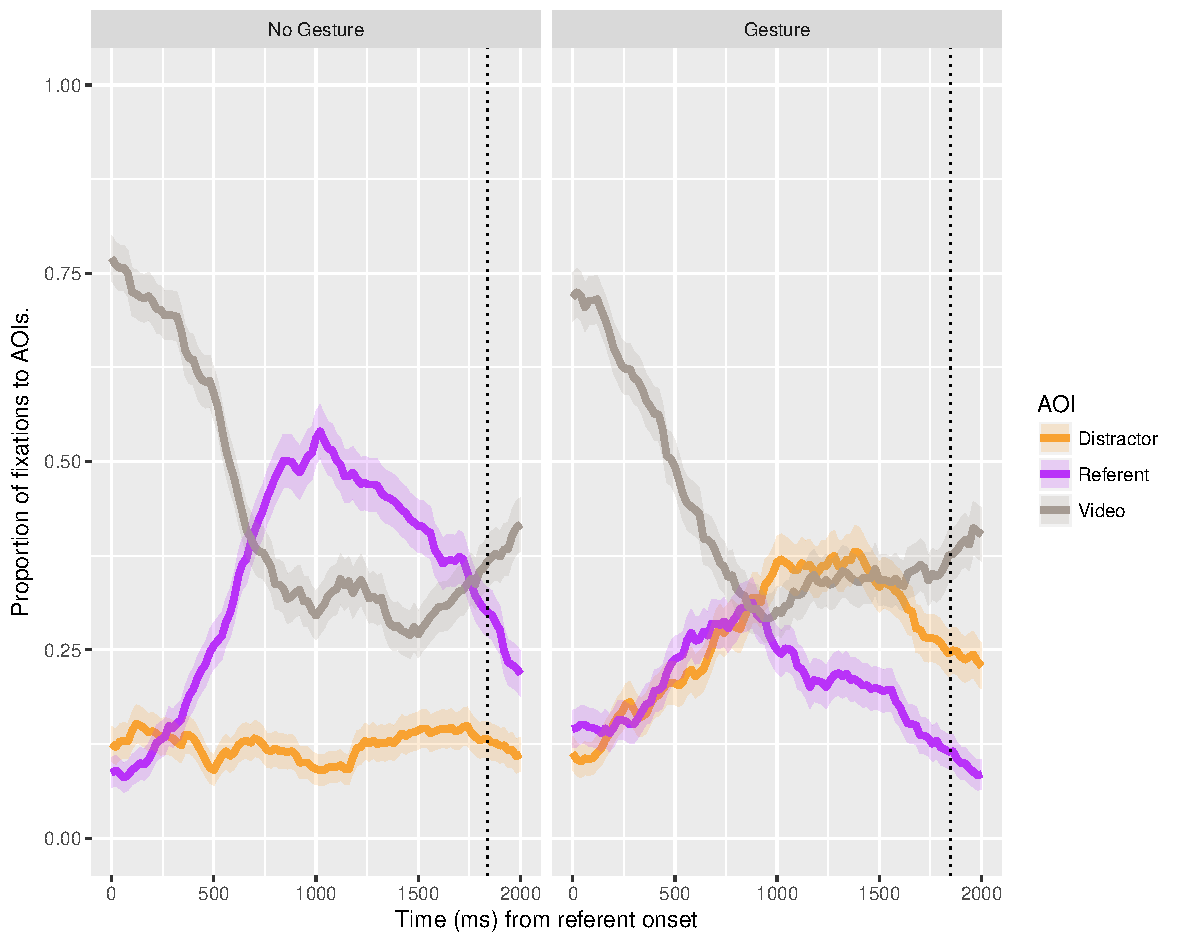
\includegraphics[width=\linewidth]{./img/e8_fixations.pdf}
  \caption{Eye-tracking results for Experiment 2: Proportion of fixations to each object (referent, distractor, video), from 0 to 2000 ms post-referent onset, calculated out of the total sum of fixations for each 20~ms time bin. Shaded areas represent $\pm$ 1 standard error of the mean.}
  \label{fig:v2_eye}
\end{figure}

%%%%%%%%%%%%%%%%%JK HERE


\subsection{Mouse movements}
Figure \ref{fig:v2_mouse} shows the time-course of the proportions of cumulative distance the mouse moved towards the referent and distractor for 2000~ms from referent onset, split by presence of cue.
Analysis on the period from 0 to 800~ms post-referent onset patterned with the eye-tracking data:
Following no-cue videos, participants showed a tendency to move the mouse increasingly towards referent over this period (\resultsLM{1.90}{0.39}{>2}).
As with eye-movements, this referent-bias was greatly reduced following an adaptor gesture (\resultsLM{-2.46}{0.77}{>2})

\begin{figure}[Ht]gesture
  \centering
	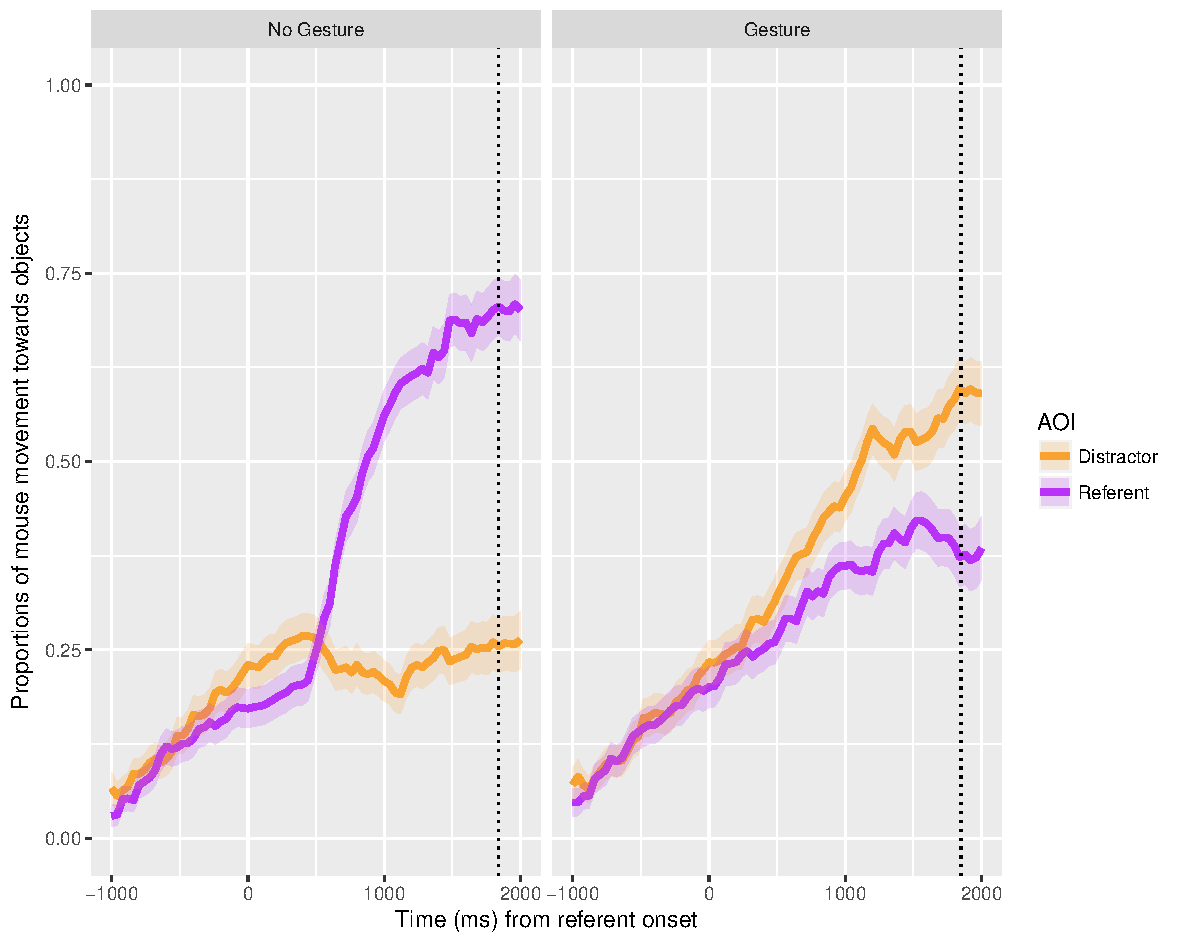
\includegraphics[width=\linewidth]{./img/e8_mouset.pdf}
  \caption{Mouse-tracking results for Experiment 2: Proportion of cumulative distance traveled toward each object from 0 to 2000 ms post-referent onset. Proportions were calculated from the total cumulative distance participants moved the mouse until that time bin (from speech-onset, when cursor was made visible). Shaded areas represent $\pm$ 1 standard error of the mean.}
  \label{fig:v2_mouse}
\end{figure}

\section{General discussion}
Across both experiments, participants showed a slight overall tendency to interpret an utterance as honest rather than dishonest, although this only differed from chance in Experiment 1. 
This bias is in line with results from previous research on deception, which shows that listeners have a general tendency to judge a speaker as truthful (\citealt{Vrij2000}). 
Utterances presented with the speaker in a neutral posture and not gesturing bias listeners towards believing the speaker to be truthful, as shown by increased tendency to fixate on, and move the mouse towards, the object which was named by the speaker. 
This result parallels the finding in \citet{Loy2017} where fluent (as opposed to disfluent) utterances saw a bias to infer the speaker to be truthful, and suggests that listeners may have an implicit honesty-bias when faced with no obvious potential cue to deception. 

Our results support the theory that the body language and movements which accompany a spoken utterance influences the judgments listeners make about the utterance's veracity.
Consistent with previous research on beliefs about and judgments based on visual cues to deception, both experiments found that participants associated an increase in movement with dishonesty \citep{Zuckerman1981}. 
Evidence for the influence of these cues was found to occur at the early stages of reference comprehension, with Experiment 2 finding that the initial bias towards the named-object over the distractor-object was completely attenuated when presented with an adaptor gesture. 
This suggests that visual information about the visual delivery of an utterance, just like spoken delivery, can modulate listeners' judgments about a speaker's intentions concurrently with the integration of lexical information.

Interestingly, in both experiments, the bias towards the distractor --- signifying perceived dishonesty --- over the referent appeared approximately 1000~ms after the referent began, at a later point than previous versions of this paradigm in which speech disfluencies were found to modulate judgments of deception. 
This, along with the fact that static videos of a speaker in different postures also influenced participants deception judgments in experiment 1, contrasts to a view of listeners relying on rule-of-thumb associations between visual cues and deception.
Our attempts to explore whether these associations are established via perceived nervousness of the speaker were inconclusive: Participant's ratings of how nervous the speaker looked in each video did not pattern with their final judgments beyond whether or not the video presented a cue, suggesting that the associations between adaptor gestures and lying patterns with, but is not necessarily a consequence of perceived anxiety in the speaker.

Our results show that the integration of the visual channel can have a rapid and direct effect on pragmatic judgements, supporting the idea that communication is fundamentally multimodal: Speech and gesture interactively codetermine meaning.
However, the integration of visual cues to inform deception judgments appears to be more gradual than the integration of spoken cues.
To better understand how cues to deception in different modalities affect comprehension, further research would require investigating the effect of spoken delivery when the visual channel is also available --- for example, studying the time course of deception judgments when faced with one or both of a disfluency and an adaptor gesture. %i.e. GVD 

\bibliography{./GCD}

\end{document}
